\documentclass[20pt, a1paper, landscape]{tikzposter}
\usepackage[utf8]{inputenc}
 
\title{Function - 8: Beta Function}
\author{Charanpreet Singh Bedi, 40048683}

\institute{Concordia University}
 
\usepackage{blindtext}
\usepackage{comment}
 
\usetheme{Simple}
 
\begin{document}
 
\maketitle

\begin{columns}
    \column{0.3}
    \block{Introduction}{Beta function is also known as Euler's integral of first kind and is very important in calculus and is basically an association between input and output values. The beta function is used to determine average time to complete some tasks in the time related problems. Beta function has a very close connection to the gamma function which also the generalisation of the factorial function. The beta function is defined as follows:
    $$\beta(x,y) =\int_{0}^{1} t^{x-1} (1-t)^{y-1} dt$$
    \newline
    \begin{itemize}
        \item Domain: Re (x) $>$ 0 and Re (y) $>$ 0
        \item Co-domain: All real numbers \[ (-\infty,\infty )\]
    \end{itemize}
    }
    \column{0.4}
    \block{Algorithm used}{
    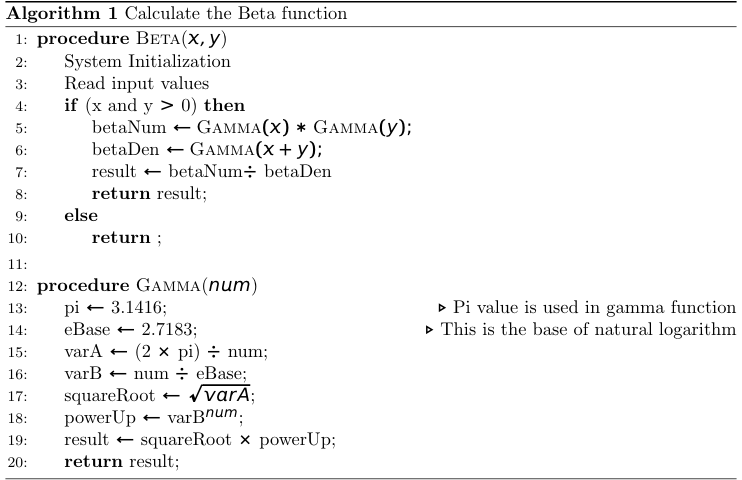
\includegraphics[]{algo.png}
    }
    \column{0.3}
    \block{Lessons Learnt}{ There were many useful lessons that were learned during development, testing and brainstorming.\newline
    \begin{itemize}
        \item Always plan the deliverable according to time in hand.
        \item Setting up meetings with the teammates and coming up with decisions that are followed by the whole team take a lot of time and input from the whole team.
        \item Follow certain coding standards, which makes it easier to understand the code and also maintain it for further integration.
    \end{itemize}
    }
\end{columns}
 
\begin{columns}
    \column{0.3}
    \block{Repository}{Throughout the brainstorming and development of the project all the files were updated and committed to the central repository. There were two repos maintained, one for the whole team (Team - A), and the other for the each individual of the team.
    \newline\newline
    Following is the address of the GitHub,\newline https://github.com/charan121317/soen-6011-project}
    \column{0.4}
    \block{Critical Decisions}{
    There were a few decisions made during the project that were very critical:\newline
    \begin{itemize}
        \item Using Gamma function to calculate beta function.
        $$\beta(x,y) = \frac{\gamma(x)\gamma(y)}{\gamma(x+y)}$$
        \item Choosing the Stirling's Approximation, to calculate the gamma function, it is an approximation for \textit{factorials}. It is very useful in calculation of gamma function, even for very small numbers.
        \item Use of MVC design pattern to make it easier to develop and maintain different modules of code.
    \end{itemize}
    }
    \column{0.3}
    \block{}{\begin{thebibliography}{}
\bibitem{Riddhi D}
Beta function and its Applications.
\textit{by Riddhi D.}
Department of Physics and Astronomy
The University of Tennessee
Knoxville, TN 37919, USA
\bibitem{wikipedia}
Wikiedia: Beta Function,
\\\texttt{https://en.wikipedia.org/wiki/Beta\_function}
\bibitem{brilliant}
Brilliant: The Beta Function,
\\\texttt{https://brilliant.org/wiki/beta-function/}
\bibitem{quora}
Quora: What is a Beta Function,
\\\texttt{https://www.quora.com/What-is-beta-function}
\end{thebibliography}}
\end{columns}
\end{document}